\documentclass[12pt, notitlepage]{article}
\usepackage[margin = 1in]{geometry}
\usepackage[english]{babel}
\usepackage[utf8]{inputenc}
\usepackage[table]{xcolor}
\usepackage{graphicx, booktabs, tikz, enumitem, dcolumn, pdfpages, csquotes}
\usepackage[font=normalsize]{caption}%,labelfont=bf
\usepackage{subcaption}
\usepackage[colorlinks = TRUE, allcolors = blue]{hyperref}

\renewcommand*\rmdefault{ppl}

\usepackage{setspace}
\setstretch{1.5}

\usepackage[]{titlesec}
    \titleformat*{\section}{\large\bf}
    \titleformat*{\subsection}{\normalsize\it}

% Bibliography
% \usepackage[natbibapa]{apacite}
\usepackage[round]{natbib}
\renewcommand{\bibliographytypesize}{\normalsize}
\setlength{\bibsep}{5pt}

\widowpenalty=10000
\clubpenalty=10000

\title{\Large Violence, co-optation, and postwar voting in Guatemala}
\author{}%Francisco Villamil\footnote{Contact: francisco.villamil@uc3m.es}\\\textit{Universidad Carlos III de Madrid}}
\date{Word count: 9,990}

% \usepackage[none]{hyphenat}

\begin{document}

\maketitle
\thispagestyle{empty}

\vspace{30pt}

\begin{abstract}
\setstretch{1.1}

Wartime civilian victimization produces a counter-reaction against the perpetrator. However, this effect hinges on the creation of collective memories of the conflict. In many countries, former fighting actors and political elites try to redirect memories of the conflict through denial, propaganda, and co-optation. Previous works have ignored these aspects. I argue that the effect of violence is conditional on the capacity of local communities to build collective memories and bypass those efforts. I test this argument using local-level from Guatemala. Results show that the effects of state violence on postwar voting depend on prewar exposure to political mobilization.

\end{abstract}
\setstretch{1.5}

\newpage
\setcounter{page}{1}

\section*{Introduction}

Conflicts leave deep scars in postwar societies, but they do not always do so the way it is usually implied.
In recent years, previous research has explored the long-term effect of civilian victimization on political preferences, showing that wartime violence against civilians produces a counter-mobilization against the perpetrator \citep{Balcells:2012aa, Lupu:2017aa, Fontana:2017aa, Rozenas:2017aa, Rozenas:2019aa}.
However, we know little about the conditions that influence the way civilians remember violent events.

In many postwar contexts, fighting actors or political elites try to steer memories of the conflict to avoid a particular reaction by the population, particularly if wartime events could be harmful for them in terms of public support.
Violence against civilians is denied, blamed on the opposite side, or interpreted as a necessary means to bring peace and national unity.
Cases like Sri Lanka or Spain show that governments sometimes impose their own interpretation of the conflict after its end, denying claims of violence against civilians or blaming them on the opposite side \citep{Seoighe:2017aa, Palomares:2004aa}.

While in some cases these efforts are not successful, in others the state is able to cover up wartime events or change collective memories of the violence.
For instance, in Argentina, people only found out about the extent of the repression carried out by the dictatorship after its defeat in 1982 \citep{Robben:1995aa}.
In addition to efforts to change the official discourse and cover up events, the co-optation of local elites and their use by state authorities---or rebel groups---is another effective strategy to avoid local counter-mobilization.
In Mozambique, \citet{Finnegan:1992aa} found that civilians who had been captives of Renamo did not show any grievances towards the \textit{majubas}, the local enforcers of Renamo, perhaps because of the personal and family links they shared.

Does wartime violence have different effects on political preferences depending on the exposure to reinterpretation efforts?
And more importantly, are some local communities better able to resist these efforts?
The theoretical framework found in previous research is not able to answer these questions, as past works do not usually account for any local factor that could mediate the long-term effect of civilian victimization.
Violence is assumed to have an homogenous effect across different communities.
This omission makes it difficult to evaluate how active efforts by the political actors involved define the actual consequences of violence.

This paper tries to address this limitation.
I argue that the effect of wartime violence is the product of a social construction of collective memories, which is influenced by both efforts by the perpetrator to stave off blame on wartime atrocities and the capacity of local communities to build the collective memories that lead to a rejection of the perpetrator.
In particular, the local ideological context, or the existence of an ideological capital that makes local communities form a political interpretation of violent events and confront propaganda efforts by the perpetrator, determines the effect of victimization on political preferences.

I focus on the case of Guatemala, which is a good example of the use of denying and cooptation strategies.
In the aftermath of the victimization campaign that took place in the early 1980s, the state tried to deny war events, set up a discourse that justified military actions as a necessary step to bring peace to the country, and co-opted the local population forcefully recruiting civilians into paramilitary units of local defense.
In a country where many areas had had limited contact with national politics and where political illiteracy was rampant, this strategy was in many cases successful.
Some of the areas that were most brutally hit by state violence during the early 1980s became years later the electoral strongholds of the right-wing political party led by the same dictator who had ordered many of the killings \citep{Ball:1999ab}.

However, I argue this was not always the case.
Some communities had been exposed to leftist political mobilization in the years prior to the most violent phase of the war.
This exposure made them more resilient to the co-optation efforts of state authorities and the discoursed imposed by the government.
Prewar political mobilization, which in this case had been mostly carried out by activists linked to the peasant movement and priests inspired by Liberation Theology, provided these communities with a better understanding of political divisions and shaped local reactions to violence.

I test this argument analyzing the local-level effect of state-led violence against civilians during the civil war on postwar vote for both the \textit{Unidad Revolucionaria Nacional Guatemalteca} (Guatemalan National Revolutionary Unity, URNG) and \textit{Frente Republicano Guatemalteco} (Guatemalan Republican Front, FRG).
While the URNG is the main political party that emerged from the former guerrilla groups, the FRG was the right-wing party founded by General Ríos Montt, who was the President of Guatemala during the early 1980s and one of the main responsible persons of the victimization campaign.
I probe whether the effect of violence on electoral support for these parties is dependent on the level of prewar exposure to political mobilization in each municipality.
Because a direct measure of prewar mobilization is not available, I use to proxies based on road infrastructure: distance to the Pan-American Highway and the local share of non-paved roads around 1970.
I assume that accessibility determined how much exposure local communities had to external political actors, who came to bring new political ideas and organize the local population.
Isolated areas only came into contact with the master cleavage as wartime violence raged their communities, and thus were more likely to accept the state's interpretation of the conflict.

The empirical analyses support these expectations.
In more accessible municipalities, and thus those that presumably were more exposed to political mobilization prior to the victimization campaign of the early 1980s, state violence is linked to an increase in electoral support for the URNG and a decrease in support for the FRG.
On the contrary, in isolated places with worse road infrastructures, state violence did not have any meaningful effect in postwar voting patterns.

This paper contributes particularly to the literature on the historical legacies of conflict \citep{Daly:2012aa, Weintraub:2015aa, Osorio:2018aa, Zhukov:2018aa, Osorio:2021aa} and the long-term effect of violence on preferences \citep{Balcells:2012aa, Lupu:2017aa, Fontana:2017aa, Rozenas:2017aa, Rozenas:2019aa} in three ways.
First, it highlights that the political reaction to wartime events is influenced by the efforts of political elites to steer memories of conflict and the capacity of individuals or communities to resist these efforts.
Second, I show that the effects of wartime violence on political preferences are not homogenous, but depend on the degree of political mobilization at the local level.
Finally, I offer new empirical evidence from a case that has received little attention in the literature, at least compared to other Latin American countries.
This study advances our understanding of the consequences of wartime violence and opens up new possibilities for future research.

\section*{Long-term effects of civilian victimization}

Building on the literature on the effects of violence on social attitudes and behavior \citep{Bauer:2016aa}, an emerging research agenda explores the long-term effects of violence against civilians.
While some works pivot around the historical legacies of conflicts on a set of different outcomes, including contemporary violent mobilization or turnout \citep{Daly:2012aa, Weintraub:2015aa, Osorio:2018aa, Zhukov:2018aa, Osorio:2021aa}, another body of research has a more explicit focus on the effects of wartime violence against civilians on political preferences.
Most of the latter find evidence for the so-called backfiring effect, in other words, that violence against civilians causes a rejection of the perpetrator's political identity in the long run.

Using data at the individual level, \citet{Balcells:2012aa} studies the long-term effect of violence in Spain.
\citet{Lupu:2017aa} do a similar study in Ukraine, tracking the inter-generational transmission of conflict-related preferences at the level of individuals.
Both these works find that violence produces a backfiring effect among those who suffered violence or their relatives.

Another set of works focuses at the level of local communities.
\citet{Balcells:2010ab} analyzes the effect of civilian victimization on local-level voting patterns in Catalonia, Spain, without finding conclusive results.
\citet{Fontana:2017aa} explore the effect of the Nazi occupation of Italy during World War II and find that Nazi violence increased local electoral support for communist parties many decades later.
\citet{Rozenas:2017aa} find that the forced deportations by Stalin that took place in Ukraine in the 1940s are linked to less support for pro-Russian political parties in the long run.

These works suffer from a few limitations.
Previous research has treated the process that leads from violent events to a change in political preferences in a too simplistic way, treating it as a black box.
A partial exception is \citet{Rozenas:2019aa}, who study the long-term effects of the Holomodor in Ukraine, and find that the effect of state repression is conditional on the structure of political opportunities.
In particular, opposition in communities exposed to repression was only visible during periods when the Soviet state could not credibly commit to repress contentious activities.

Despite its relevance, local-level conditions to the effect of violence are still missing from the explanations.
Individuals are assumed to objectively interpret violent events, and no attention is paid to those external factors that might influence this interpretation, such as propaganda or co-optation efforts by the perpetrator.
As \citet[1244]{Basta:2018aa} says, ``scholars usually take the meaning of events for granted, examining their causal efficacy without accounting for the processes of political contestation through which this meaning is created.''
Little theoretical attention has been paid to those local conditions that might explain the heterogenous effects of violence.
Empirical analyses usually compare only individuals or communities that suffered violence in the past with those that did not.

Focusing on Guatemala, the closest work to this paper is \citet{Vogt:2019aa}.
Using a similar research design, they show that state violence during the civil war in Guatemala led to higher electoral support for leftist parties in the postwar period.
They argue that the effect of violence should depend on the ``victims' embeddedness in their communities'' and show that the effect of state violence is more persistence in municipalities with a higher share of indigenous population.

However, linking the share of indigenous population to community cohesion is relatively problematic, particularly when some authors report fierce local conflicts and an increase of distrust in indigenous municipalities as a consequence of the counter-insurgency campaign \citep[e.g.][]{Burrell:2013aa}.
Two further reasons suggest caution when interpreting the results regarding the persistence of leftist electoral support.
First, state violence was more heavily concentrated in municipalities with a large share of indigenous population.
This issue could be problematic since they do not weight the number of killings by the population in each municipality.
And second, the fact that in both 2011 and 2015 elections the URNG run in a coalition with Winaq, an explicitly Indigenous party, might explain part of this persistence in indigenous areas.
In any case, these findings are not at odds with the argument of this paper, and the argument on the role of social cohesion has more to do with the persistence of political identities than with their formation as a result of witnessing violence.

This paper tries to overcome the limitations of previous works.
I assume that the process leading from violent events to a change in political preferences is not a direct, homogenous one.
The translation of wartime events into a change in preferences depends on the political interpretation of these events and the creation of collective memories of the conflict.
Efforts by the perpetrator in changing the interpretations and thus steering memories of the conflict can effectively alter the response to wartime events.
And given that the political response to events involves a social process of interpretation and remembering, the local ideological context can explain where these efforts succeed and where they fail.

In the next section I discuss the case of Guatemala and develop the theoretical expectations about the effect of wartime violence on political preferences.
My theoretical framework rests on two ideas.
First, violent events need to be depicted within a certain frame for individuals to develop a political interpretation of them.
An event of violence does not necessarily equal the account people have of it \citep{Basta:2018aa}.
Previous research has shown that different individuals can hold very different views of the same wartime events \citep{Driscoll:2016aa}, a variation that can follow political factors \citep{Silverman:2019aa}.
This is particularly relevant in a context of violence against civilians, since civilians usually cope with trauma collectively \citep{Lyons:1998aa}.

Second, the creation of collective memories that stems from the interpretation of events is a form of political socialization.
Individuals share their own interpretations of wartime events and the political response to them, giving rise to collective memories.
The type of political interpretations an individual is faced with in face-to-face interactions is probably a more important determinant of her own political response to these events than the events themselves \citep{Dyrstad:2012aa, Molina:2014aa, Glaurdic:2016aa}.
This idea speaks to previous research on the role of social contexts in the persistence of political attitudes \citep{Wittenberg:2006aa, Tavits:2013aa}.

After presenting the historical context in the next section, I build upon these two ideas and discuss two aspects of the case of Guatemala.
First, the strategies used by state authorities to co-opt the local population and avoid being blamed for the violence.
And second, how certain communities had already acquired the necessary tools to resist these efforts and develop a counter-reaction against the perpetrator.

\section*{Historical context}

The Guatemalan civil war formally started in 1960 when a group of young officers led a revolt against the US-sponsored government.
The rebel officers made contact with the urban leftist movement and formed a guerrilla group based in the rural, non-indigenous areas in eastern Guatemala \citep{Arias:1992aa}, ruling out the Maya population as a potential base of social support \citep{Smith:1990ab}.
The conflict remained at a low intensity for the next years, until a successful counterinsurgency campaign managed to put down the insurrection in the late 1960s.
Many of the rebel leaders fled into exile.

Parallel to these events, the Guatemala countryside was rapidly changing.
The Catholic Action movement started to develop strongly during the 1960s.
The foreign Catholic clergy linked to the Liberation Theology expanded throughout the country, bringing new ideas and a new style of Pastoral work that criticized economic and political discrimination \citep{Arias:1992aa, Nelson:2009aa, Stoll:1999aa}.

The conflict entered a new phase in the 1970s.
Some of the defeated rebels joined forces with a younger generation and launched a new insurgency, this time with the idea of heading to the western highlands, the traditional homeland of the Maya.
The new guerrilla leaders identified the Indigenous population as a promising source of support, due to their age-old situation of political and economic discrimination \citep{Payeras:1981aa, Arias:1992aa}.
They tried to make contact with the Catholic priests, although these contacts took place in an environment of mutual distrust \citep[e.g.][]{Manz:2004aa}.

The peasant movement was already fairly developed at this point.
It had emerged during the previous democratic period between 1944 and 1954 and, similar to Catholic Action, was fighting for land redistribution and the economic rights of the rural population \citep{Handy:1994aa, Forster:2001aa}.
It introduced new forms of economic organization, mainly cooperativism, and organized local political groups.
By the late 1970s, when the Committee for Peasant Unity (CUC) was formed, they were in contact with both the Catholic priests and the guerrilla.

With a guerrilla movement getting stronger and leftist mobilization expanding through the country, violence escalated quickly.
After 1980, all of the efforts concentrated on the armed struggle that was being waged by the four active guerrilla groups, which in 1982 would get together and form the URNG.
As the conflict entered a new phase, the Guatemalan government responded with a brutal counterinsurgency campaign.
The government focused on the civilian population that they thought constituted the base of support for the rebels, which for the most part were the rural Maya of the western highlands.
Violence intensified after 1978 and, by the early 1980s, reached genocidal levels.
More than 200,000 civilians were killed during the civil war, and over 90\% of the killings were committed by state forces \citep{Ball:1999aa, CEH:1999aa}.
% Figure \ref{fig:govt_vi_time} shows the number of state killings by year, with the most violent period (1978--1985) marked.
%
% \begin{figure*}[htb!]
%   \centering
%     \includegraphics[width = .75\textwidth]{../../../../dissertation/empirics/guatemala/govt_vi_years}
%
%   \caption{State violence against civilians in Guatemala over time} \label{fig:govt_vi_time}
%
% \end{figure*}

Civilian victimization was first carried out in a relatively haphazard way under the regime of Lucas Garcia (1978--1982).
It later became more strategic under Ríos Montt (1982--1983), who engaged in a `scorched earth' campaign and sponsored a system to ensure compliance from the local population: the Civil Defense Patrols, or \textit{Patrullas de Autodefensa Civil} (PAC).

The counterinsurgency campaign was successful.
Although it did not manage to end the conflict entirely, the strength of the rebel movement decreased significantly in the late 1980s and the war reached an impasse.
The peace talks finally culminated in a peace agreement signed in December 1996, and the guerrillas became a legal political party in 1998.
The war had ended, but its legacy endured in Guatemalan politics.

\section*{Violence, co-optation, and mobilization in Guatemala}

The victimization campaign of the early 1980s played out at the local level, pitting neighbors against neighbors and installing a climate of fear and distrust that would leave long-term consequences \citep{Burrell:2013aa}.
The government was successful in destroying Maya social organizations and gaining the cooperation of local communities, at least forcefully.
\citet[101]{Stoll:1999aa} tells how in ``Baja Verapaz, the army's reaction to CUC roadblocks was so savage that some of CUC's surviving members (...) changed sides and helped the army massacre one unarmed village after another.''

The PAC system, ``established in virtually every municipio of the western highlands between 1982 and 1983'' \citep[272]{Smith:1990ab}, was designed to ensure compliance within the countryside.
It forced local civilians to `defend' themselves from the guerrilla and, in many cases, successfully convinced them that they were on the good side and that violence and insecurity was the rebels' fault.
In more than a few instances, the PAC also assisted the army in massacring civilians.%, including in neighboring villages.
One of the goals of the PAC program was to destroy community networks and erode the trust among local people, which presumably had helped the guerrillas to organize a local base of support \citep{SaenzdeTejada:2004aa}.
As \citet[641]{Bateson:2017aa} says, ``during the Guatemalan civil war, the military made a concerted effort to socialize and re-educate the civilians of the Western Highlands.''

The co-optation strategies went beyond the local PAC militias, and the government explicitly recruited soldiers from the Maya communities into the army, including the infamous Kaibil, the elite units that carried out many of the atrocities.
A woman described to \citet[112]{Green:1995aa} ``the particularly gruesome death of her husband at the hands of the army, while behind her on the wall prominently displayed was a photograph of her son in his Kaibil uniform.''

Beyond forced recruitment, the army also purposely establish a climate of fear, which indeed ``made individuals more receptive to the military's propaganda, as they were desperate for some narrative to make sense of the chaotic, unpredictable violence surrounding them'' \citep[643]{Bateson:2017aa}.
The ideological warfare included rightist propaganda against communist ideas and any non-traditional form of social organization, blaming those activities for the violence.
Ethnic identities were the target of the campaign as well.
Given that the Maya population eventually became the social base of support sought by the rebels, the ``program [was] based on eroding ethnic identity among Guatemala's Mayan Indian majority, and on brainwashing'' \citep[21]{Black:1985aa}.

This strategy had important consequences in the long term.
The PAC system, in particular, was widely regarded by people across the political spectrum in Guatemala as the most successful element of the army counterinsurgency campaign \citep[101]{Garrard-Burnett:2010aa}.
And in any case, the whole co-optation plan and the insecurity and uncertainty that prevailed in the countryside during the 1980s helped convince the local population of the army's anti-rebel theses and left a long-term distrust for politics \citep{Green:1995aa}.

The co-optation of local people through forced collaboration is not unique to Guatemala.
Neither are the ideological consequences of counterinsurgent campaigns.
% \citet{Finnegan:1992aa} observed a similar attitude towards local paramilitary units in Mozambique.
\citet{Matanock:2018aa} show that civilians falsify their reported support for the military when asked about the counterinsurgency in Colombia, particularly in areas previously held by the insurgents.
Preference falsification helps to explain the apparent success of counterinsurgent campaigns, as fear is a major factor explaining the negative effect of repression on opposition activities \citep{Young:2019aa}.
In a study on postwar elections, \citet[749]{Daly:2019aa} says that ``the security gains attributed to the stronger belligerent offsets the belligerent's use of atrocities, allowing it largely to evade culpability for violence.''

\subsection*{The role of prewar mobilization}

The propaganda and co-optation campaign of the government was successful in building an alternative discourse of the war and shaving off culpabilities in many areas.
But not in all of them.
Some communities were better prepared to confront it than others.
Before the war, they had been more exposed to leftist ideas of political and economic discrimation, and were better equipped to understand the conflict and develop collective memories of it.
\citet[223]{Kobrak:2013aa} illustrates this argument, saying that ``living under army control, many guerrilla supporters learned to forget they had even been attracted to the struggle at all. But not in Colotenango.''
In that community, he continues, peasant organizations had been particularly strong and managed ``to challenge the mind-set of submission the army had tried to establish through the civil patrols'' \citep[226]{Kobrak:2013aa}.

Mainly two types of actors carried out these activities during the 1960s and 1970s.
On the one hand, the Catholic Action priests inspired by the Liberation Theology, which was already becoming a key political influence in Latin American \citep[e.g.][]{Wood:2003aa}.
In Guatemala, these religious activities took place at the local level throughout the countryside and had a clear political dimension, introducing the concepts and tools necessary to interpret wartime violence politically \citep{Carmack:1988aa, Manz:1988aa, Manz:2004aa, LeBot:1992aa, Bateson:2013aa}.

On the other hand, the peasant movement developed parallel to the expansion of the Liberation Theology clergy, and they eventually became deeply intertwined.
Actually, much of the work that Catholic priests carried out involved developing new forms of social and agricultural organization, namely the cooperative movement.
Cooperativism had profound political consequences since it organized the local population and show them alternative options to the existing economic and social regime \citep{Arias:1992aa, Nelson:2009aa, Bateson:2013aa}.

These activities were a key factor in developing ideological affinities in a country where many areas had not been exposed to political mobilization before.
As \citet[84]{Lofving:2005aa} affirms, ``in the population as a whole the absence of ideology and the presence of violence at the time loyalties were decided upon existed parallel to the presence of a defined cause in politically active circles.''
The consequences of the political mobilization carried out by these actors would not be limited to the conflict but also have an impact the way people remembered the conflict.

Communities with a previous history of political mobilization would have had interpreted information about the war and the reasons behind the violence differently.
Previous research points to how everyday social networks act as vectors of information during a conflict \citep{Shesterinina:2016aa} and influence the political reactions to past violence \citep{Rydgren:2007aa, Dorff:2017aa}.

I argue that communities that had been more exposed to this form of leftist mobilization before the war were more resilient to the co-optation strategies carried out by the government.
They were better equipped to understand what violence meant, to create collective memories of violent events, and to develop political identities as a response.
The consequences of this mobilization extend to the postwar period.
% Below I wrap up the discussion on the case of Guatemala and summarize my empirical observations.

\subsection*{Expectations on postwar voting}

The empirical expectation hinge upon two observations.
First, the propaganda and cooptation campaign of the Guatemalan government successfully managed to steer the memories of the conflict and avoid a counter-mobilization to its use of violence.
Second, the exception were those communities that had been exposed to leftist mobilization before the war and thus had the ideological tools needed to interpret the violence and create collective memories of it.

In the empirical analyses, I track the effects of wartime violence on postwar electoral support to two political parties: the URNG and the FRG.
While the URNG was the party that emerged out of the former guerrilla group, the FRG was the party founded by General Ríos-Montt in 1989 that represented the right-wing nationalism put forward by the army during the conflict.
Even though more parties share the ideology of these two parties, these were probable the two parties more representative of the wartime cleavage.
In the appendix, however, I also include results including more political parties, particularly adding vote share for the FRG together with the \textit{Partido Patriota} (Patriot Party, PP), another right-wing, nationalist party founded in 2001 by a former army officer, Otto Pérez Molina.

Following the argument, the expectation is that state violence during the conflict should have produced a counter-reaction in the form of increased support for the URNG and decreased support for the FRG, but only in those communities where they were able to interpret the violent events and create collective memories.
The following hypotheses summarize this idea.

\begin{enumerate}[label={\bf H\arabic*:} , ref=H\arabic* , wide=0.5em, leftmargin=*]
  \item \label{h:urng-mob} In municipalities exposed to prewar political mobilization, wartime violence against civilians increased long-term local support for the URNG.
  \item \label{h:frg-mob} In municipalities exposed to prewar political mobilization, wartime violence against civilians decreased long-term local support for the FRG.
\end{enumerate}

On the contrary, in communities that had not been exposed to prewar leftist mobilization, the state should have been able to successfully co-opt the local population and avoid being blamed for the violence.
In some cases it might even be able to blame the guerrillas for the atrocities that took place during the conflict.
This meant that violence did not have any effect or even that it had the opposite one: increased support for the FRG and a rejection of the URNG.
Following this, I outline the other two hypotheses.

\begin{enumerate}[label={\bf H\arabic*:} , ref=H\arabic* , wide=0.5em, leftmargin=*]
  \setcounter{enumi}{2}
  \item \label{h:urng-no-mob} In municipalities not exposed to prewar political mobilization, wartime violence against civilians decreased long-term local support for the URNG.
  \item \label{h:frg-no-mob} In municipalities not exposed to prewar political mobilization, wartime violence against civilians increased long-term local support for the FRG.
\end{enumerate}

\section*{Empirical design}

I build a local-level dataset covering all 325 municipalities in Guatemala across the 22 departments.\footnote{Although Guatemala currently has 340 municipalities, the sample is reduced because of the territorial changes that municipalities have experienced since 1970. New municipalities were merged with the ones they once formed part of, as shown in the appendix.}
With this setup, I analyze the effect of wartime violence against civilians committed by state authorities on postwar electoral support for the URNG and FRG, adding an interaction term for the level of prewar exposure to leftist mobilization.

I run OLS models pooling observations from every municipality in all five general elections between 1999 and 2015, including election-year fixed effects.
I show models using separate cross-sectional data for each election in the appendix.
All models include department fixed effects to compare only municipalities within the same department.
Given that wartime violence was strongly concentrated in a few areas of the country, I also run the main models using a subset of the most affected departments.

\subsection*{Electoral results}

The main dependent variables are the share of votes to the URNG and the FRG in each election.
The URNG, which became a political party in 1998, was originally founded in 1982 as the umbrella group that included the four main rebel groups fighting against the government at the time.
This variable should capture pretty well the sympathy for the former rebels and, more generally, for the leftist ideology they represented.

The FRG was created in 1989 by General Efraín Ríos-Montt, the president of Guatemala between 1982 and 1983 who was behind much of the victimization campaign and designed the civil patrol system.
The FRG represented the anti-communist, right-wing nationalism that the army had sponsored during the war.
It still maintained the view that the conflict, and the violence it enfolded, had been the guerrillas' fault.

Using data from the Supreme Electoral Tribunal \citep{TSE:2019aa}, I calculated the share of total valid votes received by each party in each municipality in every election between 1999 and 2015.\footnote{The FRG did not participate in 2011 elections. The URNG share includes its coalition partners: DIA in 1999; WINAQ, ANN, and MNR in 2011; WINAQ in 2015.}
In the appendix I also include results using as the dependent variable the added electoral share of FRG and PP.\footnote{In 2011 elections, this variable only includes electoral share for the PP, as the FRG did not participate in election. The opposite happens in 1999, when only the FRG is included, as the PP was founded in 2001.}
Table \ref{tab:elec_results} shows the share of total votes received by both parties in each election.
% Their best result was in 1999 when, arguably, wartime divisions were at its height.
Figure \ref{fig:map_elec1999} shows the geographical variation in support for each party in 1999 elections.

\begin{figure*}[!ht]
    \centering

    \begin{minipage}{1\textwidth}
      \centering
      \subfloat[URNG]
        {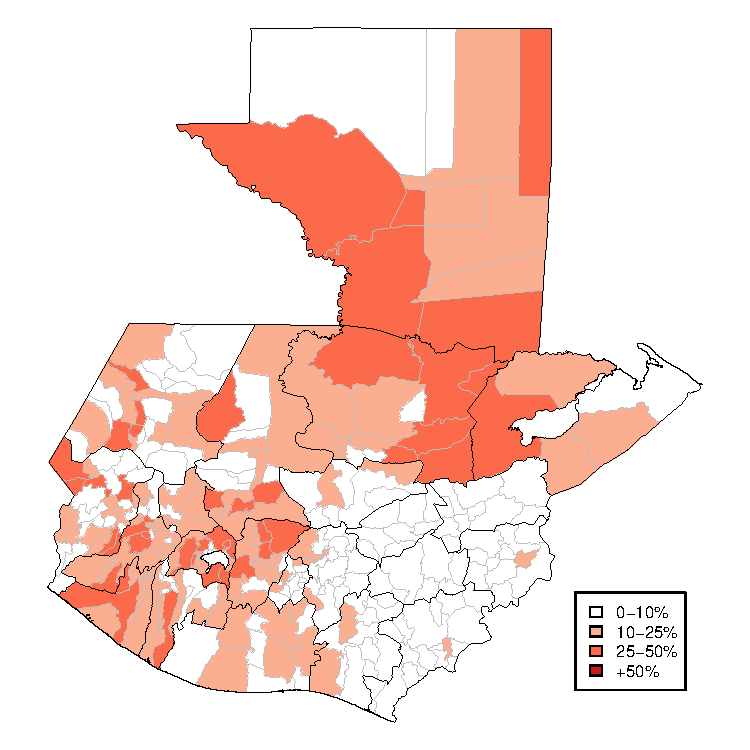
\includegraphics[width=0.4\textwidth]{../../../../dissertation/empirics/guatemala/map_URNG1999}}\hspace{25pt}
      \subfloat[FRG]
        {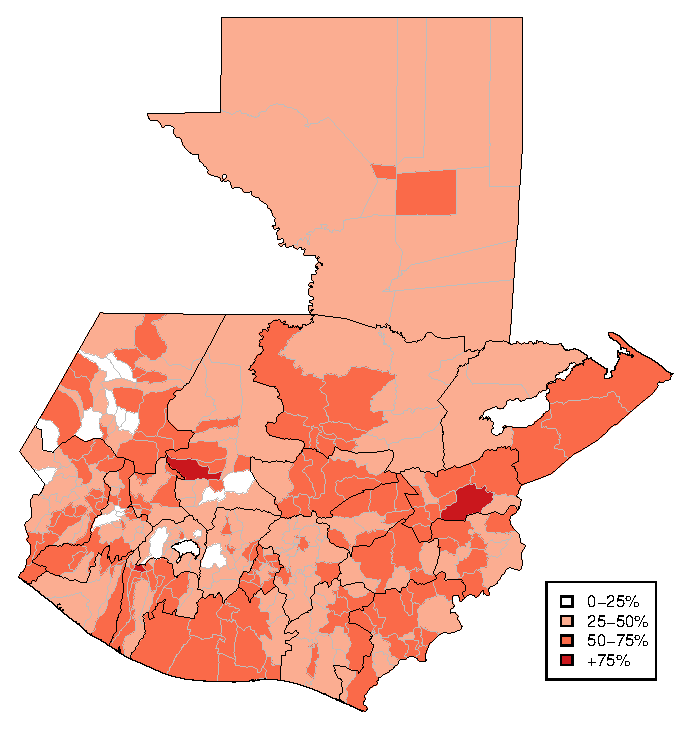
\includegraphics[width=0.4\textwidth]{../../../../dissertation/empirics/guatemala/map_FRG1999}}
    \end{minipage}

    \caption{Electoral results in 1999} \label{fig:map_elec1999}

\end{figure*}

\vspace{15pt}
\begin{table}[!htbp] \centering
  \caption{Electoral results of URNG and FRG}
  \label{tab:elec_results}
\small
  \begin{tabular}{lccccc}
  \\[-1.8ex]\hline
  \hline \\[-1.8ex]
    & 1999 & 2003 & 2007 & 2011 & 2015 \\
  \hline \\[-1.8ex]
  \input{../../../../dissertation/empirics/guatemala/nat_results_tab_URNGrow.tex}
  \input{../../../../dissertation/empirics/guatemala/nat_results_tab_FRGrow.tex}
  \hline
  \hline \\[-1.8ex]
  % \multicolumn{6}{p{9cm}}{\textit{Note:} In 2015, FRG had been renamed as PRI. Coalition partners of URNG: DIA in 1999; WINAQ, ANN, and MNR in 2011; WINAQ in 2015.}
  \end{tabular}
\end{table}

\subsection*{Civilian victimization}

To gather data on wartime violence against civilians I rely on and merge two different datasets, the records of the CEH and the \textit{Centro Internacional para Investigaciones en Derechos Humanos} (International Center for Human Rights Investigations, CIIDH), following previous research on political violence in Guatemala \citep{Chamarbagwala:2011aa, Sullivan:2012aa}.
Both CEH and CIIDH datasets are event databases built after extensive field research and together constitute a comprehensive picture of victimization events throughout the Guatemalan Civil War.

The CIIDH is a Guatemala-based NGO that carried out thousands of interviews and reviewed a variety of secondary sources to produce a list of more than 17,000 human rights violations by both sides, including more than 40,000 killings \citep{Ball:1999aa}.
The CEH was a UN-sponsored truth commission that focused on the massacres committed by the government against the civilian population and revealed that over 200,000 civilians were killed or disappeared during the conflict and that over 90\% of the killings had been committed by state authorities or related paramilitary groups \citep{CEH:1999aa}.
The CEH data was obtained from the replication data for \citet{Sullivan:2012aa}, who hand-coded massacres, defined as events of indiscriminate violence where at least 5 people were killed, from the CEH reports.

Even though the CIIDH claims that its data are not a representative sample of wartime violent events, combining it with the CEH does offer a comprehensive picture of the conflict events in Guatemala.
As \citet[382]{Sullivan:2012aa} explains, ``the three sources used to generate the CIIDH/CEH data (...) present a more accurate portrayal of the distribution of violence across Guatemala than any one source would have on its own.''
In any case, I include in the appendix results using only data from the CEH.
There are not significant changes.

In every case, only events of fatal violence against civilians were selected and those whose location was unknown were removed (0.1\% of all events).
In the analyses, data on violence against civilians is limited to the period 1978--1985, which was by far the most violent period of the conflict.% (see figure \ref{fig:govt_vi_time}).
I also include violence committed by the civil patrols, although the army participated in 98\% of the killings during this period.

For each municipality, I calculate the number of killings by state forces for every 1,000 inhabitants (using 1973 census data), and include it in the models in logarithmic form.
Figure \ref{fig:map_govt_vi} shows the geographical distribution of state violence.

\begin{figure*}[htb!]
  \centering
    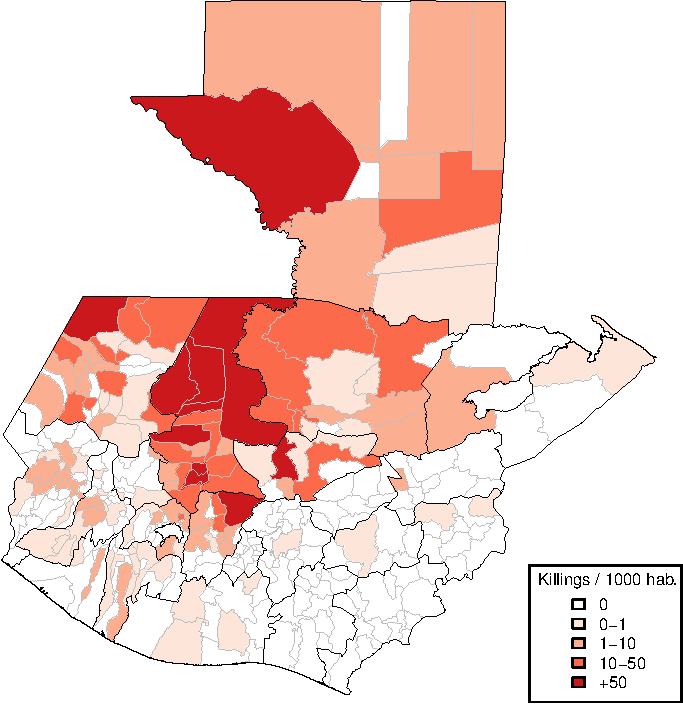
\includegraphics[width = .4\textwidth]{../../../../dissertation/empirics/guatemala/map_govt_vi}

  \caption{State violence against civilians in Guatemala, 1978--1985} \label{fig:map_govt_vi}

\end{figure*}

\subsection*{Proxying prewar mobilization}

Prewar exposure to political mobilization was a major factor determining the response of civilians to state violence in Guatemala.
Ideally, data on the presence and activities of leftist political actors---mainly peasant organizations and Liberation Theology priests---before the most intense phase of the conflict would help testing this mechanism.
However, to my best knowledge, such data is not available.
Data on other prewar activities or the extent of political mobilization at the local level is not available, either.

Instead, I use two proxies for prewar exposure to political mobilization based on road infrastructure.
In particular, I assume that accessibility in terms of road infrastructure determined how much exposure local communities had to these external political actors, who expanded throughout the country from the capital and main cities to bring new political ideas and organize the local population.

This variable is also related to state building.
My argument suggests that communities more accessible to the centers of power should be more familiar with political cleavages and thus have a higher `ideological capital.'
Thus, beyond the concrete activities of political activists, the results are also measuring the different effects of violence depending on the degree of exposure to national politics, which should go hand-in-hand with state building.
The fact that some activists and priests were actually targeting isolated areas in Guatemala for their activities is not at odds with the idea that more accessible areas should have had a more continuous and profound exposure to political mobilization.

I use two different variables based on road infrastructure: distance to the Pan-American Highway, a major road-building project completed in the 1960s, and the share of non-paved roads in each municipality around 1970.\footnote{I use the share of non-paved roads, rather than its opposite, to facilitate the interpretation of the coefficients in the regression tables.}
Neither of these two variables is correlated with patterns of state or rebel violence during the civil war, as I show in the appendix.
The most clear source of concern would be that accessibility drives rebel mobilization, which in turn would increase postwar electoral support for the rebels.
But the relationship between accessibility and rebel support through this mechanism would probably run the opposite way: state reach would decrease in more isolated areas, facilitating rebel activity.
This bias would reduce the observed relationships, rather than confound it.
Moreover, given that they are not highly correlated among them ($\rho = 0.23$), the use of two variables provides two different proxies of accessibility, increasing the validity of the results.

The Pan-American Highway was a major US-sponsored development project completed in the 1960s.
The construction of the highway greatly improved communications.
This was particularly true in countries like Guatemala where former connections consisted of dirt roads or even mule trails, impassable during the rainy season.
The Pan-American Highway crosses Guatemala from West to East, and extends through the heart of the western highlands.
The location of the route, originally planned to follow the Pacific coast, was chosen because of comercial reasons \citep{Rutkow:2019aa}.
The final construction of the highway brought about a great improvement in transportation in the early 1960s.
Precisely the moment in time when peasant associations and priests linked to the Liberation Theology began to expand throughout the country.

The assumption I make here is that municipalities closer to the Pan-American Highway had a more intense exposure to these mobilization activities due to the easier logistics of arriving to these areas.
In order words, I assume that better transport infrastructure facilitated over time the continuous arrival of more political actors from Guatemala City and abroad.
I calculate how far away each municipality is from the road, and expect that municipalities closer to the Highway had a stronger exposure to leftist political mobilization during the 1960s and early 1970s.\footnote{Source: Email communication with the National Geographic Institute of Guatemala.}
Figure \ref{fig:map_panam} shows the final measure, indicating the distance between the boundary of each municipality and the Pan-American Highway (shown as a blue line). In the analyses, this variable is used in its logarithmic form, i.e. $log(km + 1)$.

\begin{figure*}[htb!]
  \centering
    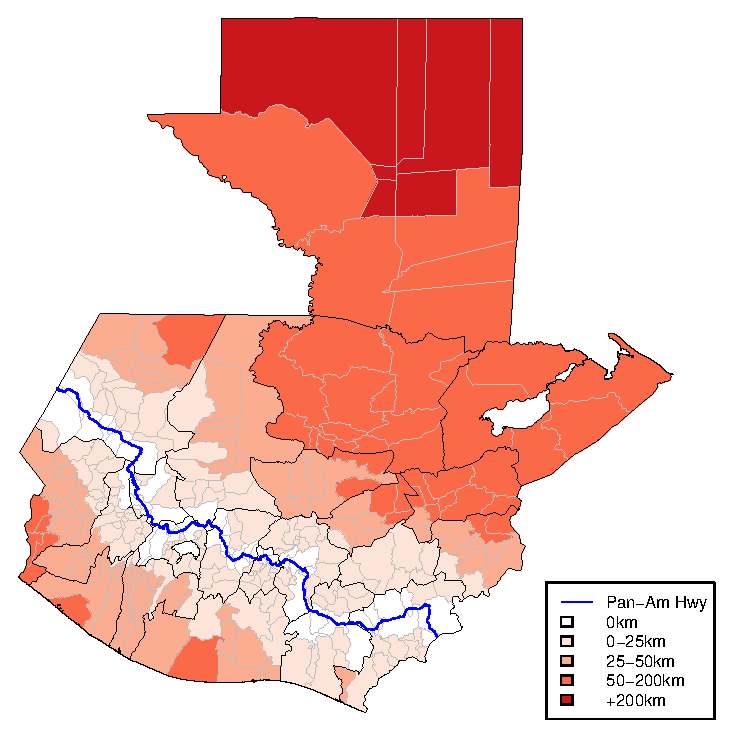
\includegraphics[width = .4\textwidth]{../../../../dissertation/empirics/guatemala/map_panam}

  \caption{Distance to Pan-American Highway} \label{fig:map_panam}

\end{figure*}

Distance to the Pan-American Highway provides more exogenous variation since the location of the highway did not response to local political dynamics.
However, it might leave out some variation across municipalities further away from the highway.
The second proxy complements this variable and offers a measure more comparable across different departments, even if it might be more correlated with local confounders.

The second variable I use to measure accessibility is the share of non-paved roads in each municipality.
Assuming that political actors would go beyond areas adjacent to the Pan-American Highway, local road infrastructure would facilitate transportation within a community, thus leading to generally higher exposure to the activities of these actors.

Data comes from the National Geographic Institute of Guatemala \citep{Segeplan:2019aa} and corresponds to the road network existent around 1970.
Although the specific date could not be found, the data is based on raw information from the 1960s and 1970s.
It constitutes the best approximation for the period of interest, namely, road infrastructure right before the conflict escalated in the late 1970s.

The left panel (a) in figure \ref{fig:map_roads} shows the road network in Guatemala, with non-paved roads in grey and paved roads in black.
The right panel (b) shows the variable used in the analyses, which calculates the share of non-paved roads out of the total length of existing roads.
I use the share of non-paved roads instead of the total length to keep a measure that is independent from the territorial extension of each municipality.

\begin{figure*}[!ht]
    \centering

    \begin{minipage}{1\textwidth}
      \centering
      \subfloat[Road network ca. 1970]
        {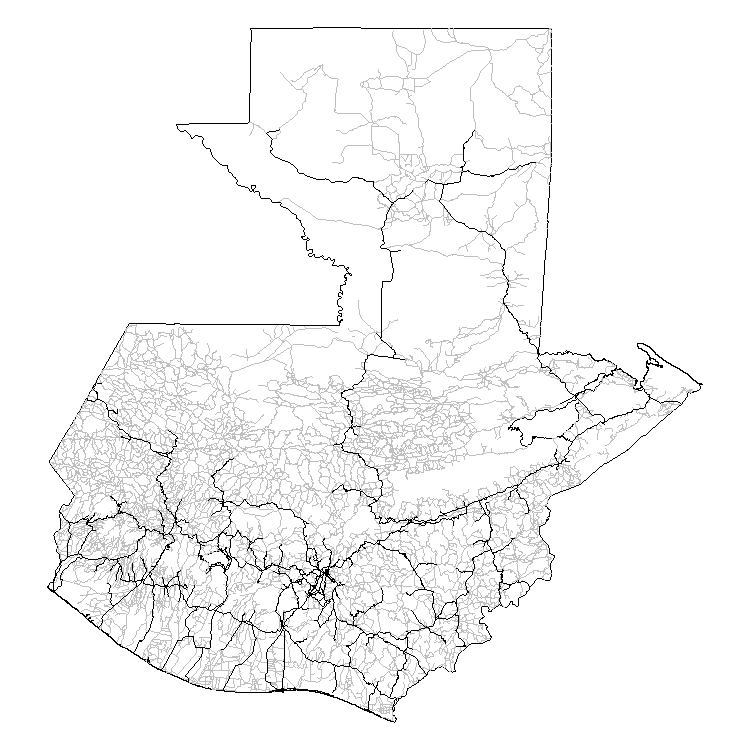
\includegraphics[width=0.4\textwidth]{../../../../dissertation/empirics/guatemala/map_roads}}\hspace{25pt}
      \subfloat[\% Non-paved by municipality]
        {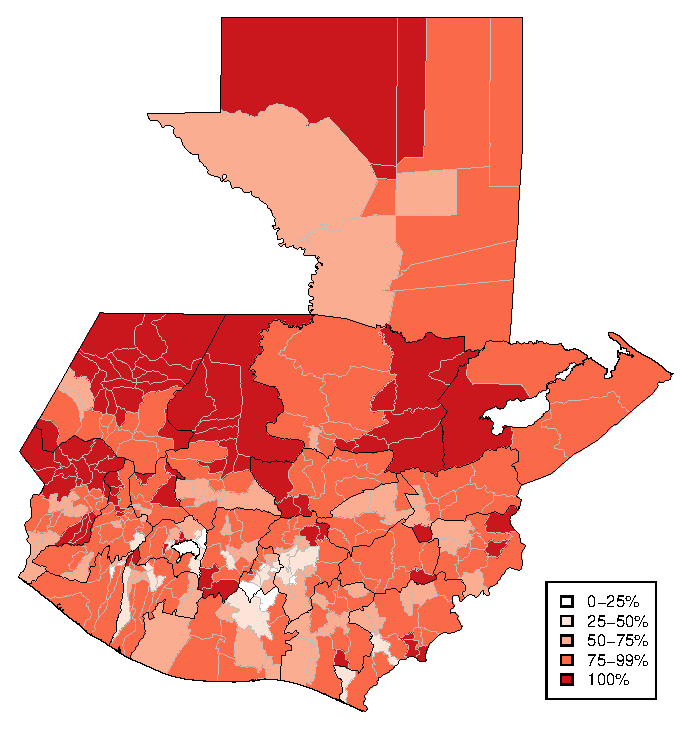
\includegraphics[width=0.4\textwidth]{../../../../dissertation/empirics/guatemala/map_roads_nonpaved_sh}}
    \end{minipage}

    \caption{Local road infrastructure} \label{fig:map_roads}

\end{figure*}

\subsection*{Controls}

Using data from the 1973 census, obtained from the replication data for \citet{Sullivan:2012aa}, I include the logged population of each municipality and the share of indigenous population.
I include two measures of terrain ruggedness, which strongly influenced the degree of wartime victimization and presence of the rebel groups during the war.
Using data from from the Digital Elevation Map of Guatemala \citep{Mapzen:2018aa} I calculate the standard deviation of elevation within each municipality, and include the share of forest cover from the GlobCover Land Cover Maps \citep{Arino:2012aa}.
I include a measure of rebel violence prior to 1978, the logged number of killings for every 1000 inhabitants following the CIIDH dataset \citep{Ball:1999aa}, to control for early rebel presence.
I also include the logged distance to Guatemala City from each municipality (in km) and the logged area of each municipality (in $km^2$).

\section*{Results}

Table \ref{tab-gt:base_models} shows the results of the base models, i.e. those that analyze the relationship between state violence and vote for the URNG and the FRG, in both the whole sample and only in the departments most affected by the violence.
In every case the data pools together observations from all elections.
The first column (1) shows a positive relationship between state-led killings and URNG vote, but no relationship in the case of the FRG (column 2).
Moreover, in both cases the election dummies show that vote for URNG and FRG was much higher in the 1999 elections.

\input{../../../../dissertation/empirics/guatemala/table_base_pooled2.tex} % tab-gt:base_models


When looking at the most affected departments, the effect of state violence on leftist vote decreases, and it only stays significant at the 90\% level.
It suggests that the general trend found in the first model could indicate a concentration on both violence and leftist vote in the western highlands and Petén, without not a robust relationship across the whole country.

Table \ref{tab-gt:int_panam} replicates the previous models but includes the interaction between state violence and the first proxy for prewar mobilization, distance to the Pan-American Highway.
In the case of URNG vote, the effect of state violence in municipalities contiguous to the highway is much stronger than in the base model.
The effect remains virtually the same in the sample limited to the most affected departments.
As the distance from the Pan-American Highway increases, the effect of state violence on leftist vote decreases.
Moreover, in the absence of violence, being closer to or further away from the highway does not have any effect on URNG vote.

\input{../../../../dissertation/empirics/guatemala/table_dist_panam2.tex} % tab-gt:int_panam

These results can be more clearly seen in figure \ref{fig:pp_urng_panam}, which shows the predicted effect of state violence on URNG vote in three municipalities located next to the highway, 20km away, and 400km away.
All other variables are kept at their mean.
State violence has a positive impact on leftist vote in the first case, but it decreases and even becomes negative as distance increases.
Assuming the variable is a good proxy for prewar mobilization, these results indicate that state violence only increased leftist vote in municipalities that had been exposed to political mobilization before the conflict intensified.

\begin{figure*}[htb!]
  \centering
    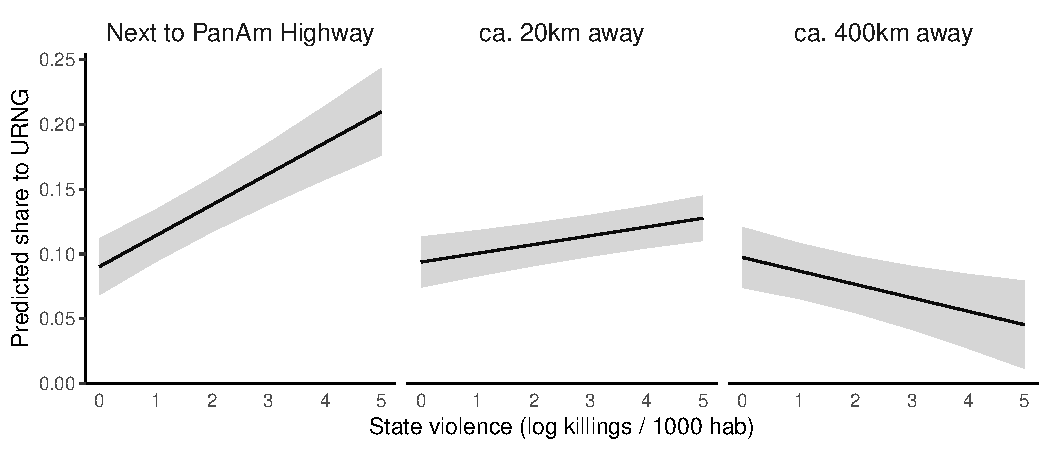
\includegraphics[width = .75\textwidth]{../../../../dissertation/empirics/guatemala/pp_urng_panam}

  \caption{Wartime state violence and URNG share depending on prewar political mobilization (proxied by distance to Pan-American Highway)} \label{fig:pp_urng_panam}

  % \vspace{5pt}
  % \raggedright
  % \scriptsize{Predicted share of URNG in the postwar period depending on wartime state violence and road infrastructure (distance to Pan-American Highway). Model includes department and election FEs. Predicted probabilities calculated for a municipality in Quiché, in 1999 elections, keeping all other variables at their mean.}

\end{figure*}

In the case of FRG vote, however, the results are not statistically significant.
State violence does not seem to have any meaningful effect, regardless of the value of the proxy for prewar mobilization.
Figure \ref{fig:pp_frg_panam} illustrates this result, showing that, if anything, the results for the FRG go in the opposite direction that the the models explaining URNG vote.

\begin{figure*}[htb!]
  \centering
    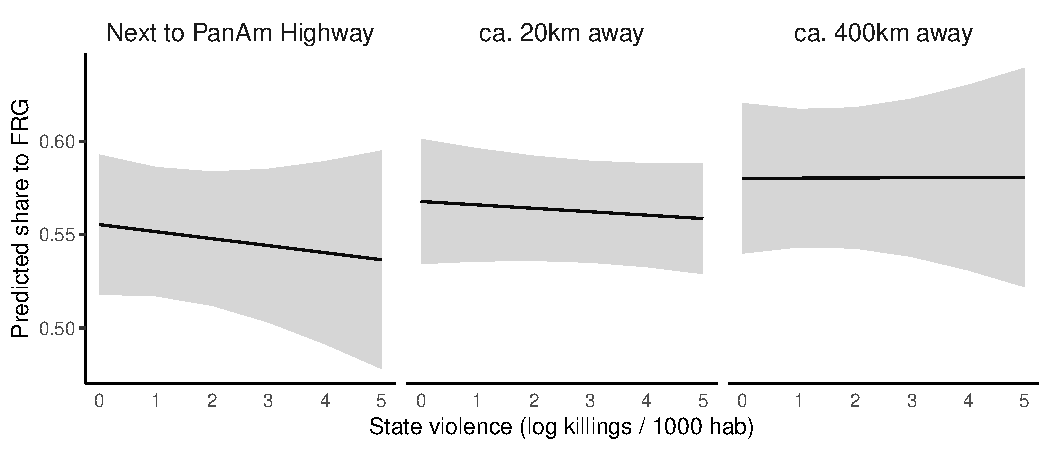
\includegraphics[width = .75\textwidth]{../../../../dissertation/empirics/guatemala/pp_frg_panam}

  \caption{Wartime state violence and FRG share depending on prewar political mobilization (proxied by distance to Pan-American Highway)} \label{fig:pp_frg_panam}

  % \vspace{5pt}
  % \raggedright
  % \scriptsize{Predicted share of FRG in the postwar period depending on wartime state violence and road infrastructure (distance to Pan-American Highway). Model includes department and election FEs. Predicted probabilities calculated for a municipality in Quiché, in 1999 elections, keeping all other variables at their mean.}

\end{figure*}

Table \ref{tab-gt:int_roads} shows the results for the equivalent models substituting distance to the Pan-American Highway with the local share of non-paved roads, as the alternative accessibility proxy for prewar mobilization.
The results are stronger than those that rely on the previous variable.
State violence has a large positive effect on URNG vote in those municipalities which have all roads paved, and as the share of non-paved roads increases, the effect of state violence disappears.
In the most affected departments, the relationship is even stronger, and remains significant at the 99.9\% level.
The models on FRG vote share mirror these results but in the opposite direction, although the effect is only significant at the 95\% level.
State violence is linked to less votes for the FRG in municipalities where most roads are paved. As the share of non-paved roads increases, this effect disappears.

\input{../../../../dissertation/empirics/guatemala/table_roads_nonpaved2.tex} % tab-gt:int_roads

These results are illustrated in figures \ref{fig:pp_urng_roads} and \ref{fig:pp_frg_roads}.
State violence has a large effect on leftist vote in more accessible municipalities.
When going from 0 killings to around 150 killings per 1000 inhabitants, the expected vote for URNG rises from 10\% to more than 30\%.
In the case of FRG vote, the effect goes in the opposite direction, less robust but still significant.
Violence decreases FRG vote in municipalities where most roads are paved, while it has no effect in more isolated municipalities.

\begin{figure*}[htb!]
  \centering
    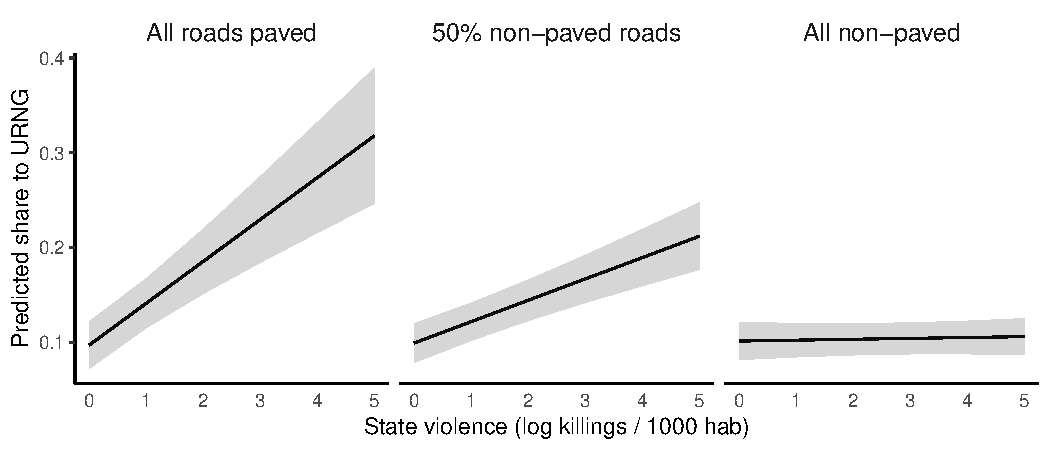
\includegraphics[width = .75\textwidth]{../../../../dissertation/empirics/guatemala/pp_urng_roads}

  \caption{Wartime state violence and URNG share depending on prewar political mobilization (proxied by \% non-paved roads)} \label{fig:pp_urng_roads}

  % \vspace{5pt}
  % \raggedright
  % \scriptsize{Predicted share of URNG in the postwar period depending on wartime state violence and road infrastructure (\% non-paved roads in a given municipality). Model includes department and election FEs. Predicted probabilities calculated for a municipality in Quiché, in 1999 elections, keeping all other variables at their mean.}

\end{figure*}

\begin{figure*}[htb!]
  \centering
    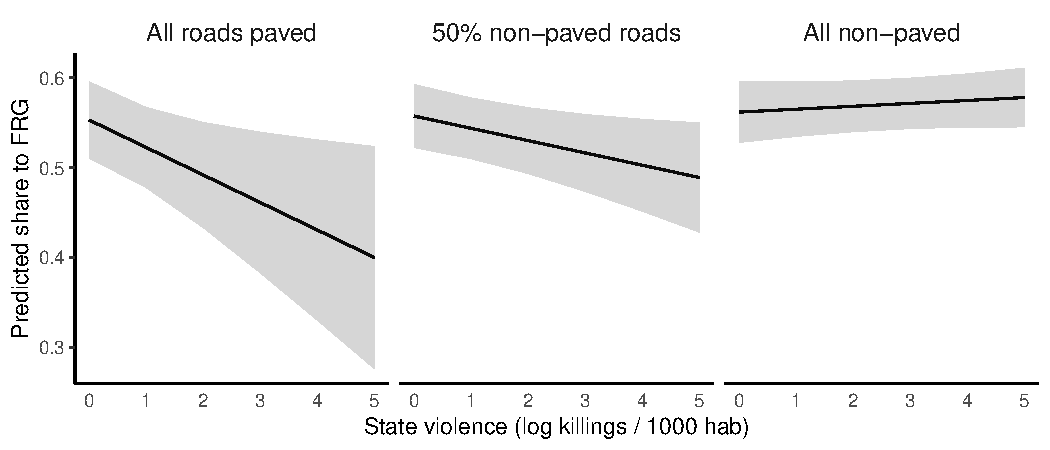
\includegraphics[width = .75\textwidth]{../../../../dissertation/empirics/guatemala/pp_frg_roads}

  \caption{Wartime state violence and FRG share depending on prewar political mobilization (proxied by \% non-paved roads)} \label{fig:pp_frg_roads}

  % \vspace{5pt}
  % \raggedright
  % \scriptsize{Predicted share of FRG in the postwar period depending on wartime state violence and road infrastructure (\% non-paved roads in a given municipality). Model includes department and election FEs. Predicted probabilities calculated for a municipality in Quiché, in 1999 elections, keeping all other variables at their mean.}

\end{figure*}

In the appendix, I show that the results do not change if the independent variable measuring wartime violence only includes data from CEH.
I also show results using, instead of FRG vote, a measure of combined electoral support for the FRG and the PP.
Finally, I include results using a cross-section of the data for each election.

The results are in line with the hypotheses outlined in the previous section, and particularly with those that refer to URNG vote (\ref{h:urng-mob} and \ref{h:urng-no-mob}).
In the case of the FRG hypotheses, the results are mixed.
The analyses provide empirical evidence for hypothesis \ref{h:frg-mob}, which predicts a decreasing effect of violence on support for the FRG in municipalities more exposed to prewar mobilization.
However, hypothesis \ref{h:frg-no-mob} is not directly supported by the data.
The expectation was that in municipalities not exposed to prewar mobilization, state violence should have been successful in increasing support for its political project (represented by the FRG).
The results show the there is no effect in this case.

\subsection*{Accessibility and violence against civilians}

An important assumption made in these analyses is that the accessibility variables are a good proxy for the level of exposure to prewar mobilization.
A quantitative test of this assumption is impossible given the absence of relevant data.
But another source of concern is that these two proxies could be related to patterns of violence against civilians.
In the appendix, I show that neither of these two variables is correlated with wartime violence by the state or the rebels.
If anything, the analyses show that wartime state violence was slightly more intense in municipalities further away from the Pan-American Highway.
Thus, none of the two proxies seems to be related to local conflict intensity.

\section*{Conclusion}

In many conflicts, political actors actively try to alter the memories of the conflict.
Propaganda, co-optation strategies, and local processes of mobilization define the political response to violence in each community.
In this paper I point to the importance of these overlooked dynamics in understanding the legacies of conflict.

Using local-level data from Guatemala, I show that in many areas the government managed not to be blamed for the brutal campaign of victimization carried out during the civil war.
However, some communities had been exposed to leftist political mobilization right before the war.
They had acquired the ideological capital necessary to interpret violent events in political terms and were more resilient to state propaganda.
In the contrary to the other areas, in these communities state violence backfired in the form of long-term support for the rebels.

% This study offers novels insights that motivate future research and inform policy-making.
Even though this study focuses on Guatemala, the insights here motivate future research and inform policy-making.
The main takeaway is that we should take into account the social processes that determine the consequences of violence.
A better understanding of the social and political legacies of conflict is of major importance for postwar societies.
In these contexts, the main goal is to avoid a new outbreak.
Knowing how violence might have heterogenous effects across different areas of the country can help to identify potential hot-spots of radicalization.
Moreover, the fact that memories of a conflict and the political responses to it are sensitive to the efforts of different political actors to change them can help to avoid such radicalization and to promote reconciliation.
A wrong reading of these findings would be that hiding facts could be a good strategy to avoid further violence.
But we do know little about how differential access to information about the conflict can bring about polirization, which constitutes a potential avenue for future research.
Instead, the discussion here suggests that peacebuilding programs should monitor the translation of collective memories into political responses and how these can lead to polarized identities.
In an unstable context, even a small fire can quickly grow in size and ignite another outbreak of violence.

\clearpage
\bibliographystyle{jpr}
\bibliography{$HOME/Documents/REF}$

% \newpage
% 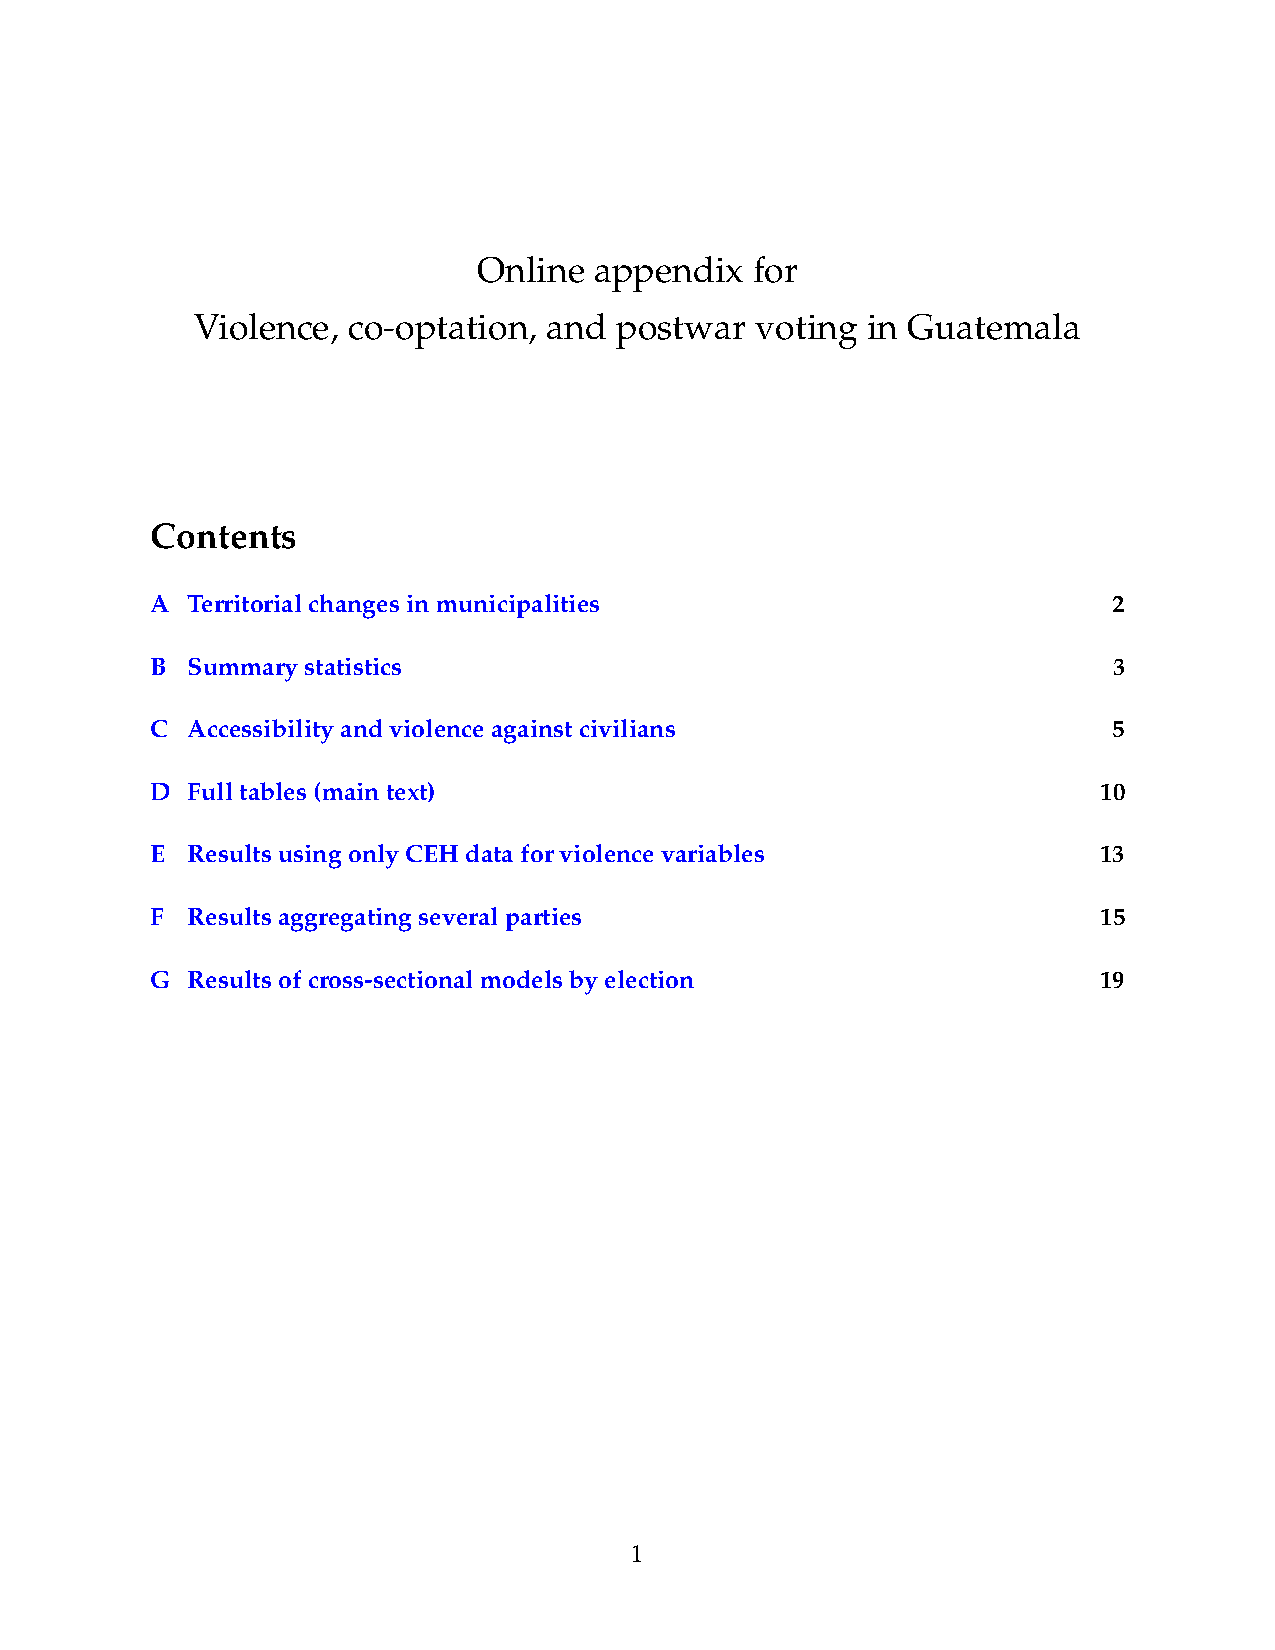
\includepdf[pages=-]{appendix.pdf}

\end{document}
